\subsection{Problem}

\renewcommand{\theequation}{\theenumi}
\begin{enumerate}[label=\thesection.\arabic*.,ref=\thesection.\theenumi]
\numberwithin{equation}{enumi}
\item Solve $\vec{x+y}<5$ graphically.
The following python code computes the graphical representation of $\vec{x+y}<5$ as shown in Fig.\ref{fig:qsix}.
	\begin{lstlisting}
	./codes/lines/q6.py
	\end{lstlisting}
	\begin{figure}[!ht]
	\centering
	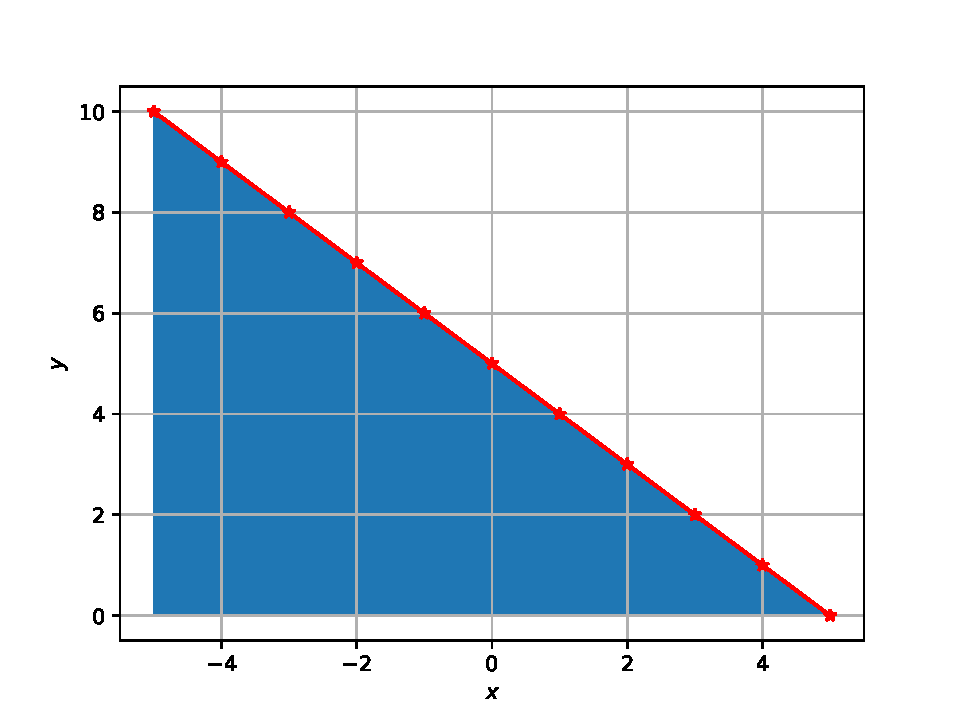
\includegraphics[width=\columnwidth]{./figs/lines/q6.pdf}
	\caption{x+y$<$5}
	\label{fig:qsix}	
	\end{figure}
	
\end{enumerate}
